\chapter{Estado del arte}
En esta sección se van a presentar algunos de los hipervisores más populares utilizados en sistemas embebidos y sus características principales, poniendo más énfasis en los casos de Xen y Jailhouse ya que se tratan de los hipervisores que se han utilizado para obtener los resultados del actual TFM. Estos dos últimos resultan de mayor interés debido a que son de código abierto, por lo que aparte de la documentación oficial, a veces un poco escasa en los proyectos de código abierto, exiten repositorios públicos con el código fuente. De esta forma, se puede realizar un mejor análisis de su estructura e incluso modificar partes de su código para adaptarlo a las necesidades del sistema.

\section{OKL4 Hypervisor}
OKL4 Hypervisor \cite{okl4} es un hipervisor de tipo 1 de los basados en micro-kernel. Fue desarrollado originalmente por OK Labs, la cual forma parte del conglomerado General Dynamics, aprovechando la experiencia en micro-kernels que habían desarrollado gracias al éxito comercial de otro de los productos de OK Labs, el micro-kernel seL4 \cite{seL4}. En su visión, no existían razones para no poder combinar en una única implementación un micro-kernel y un hipervisor. De echo, durante mucho tiempo, el OKL4 se denominó \textit{OKL4 Microvisor}.\\
El objetivo es asistir a la virtualización con la mínima sobrecarga del sistema. De esa forma, el modelo propuesto se basa en los siguientes principios:
\begin{itemize}
  \item La abstracción del sistema que el hipervisor presenta a los sistemas operativos guest consta de una o varias CPUs virtuales (\acrshort{vCPU}), en las que poder desplegar las tareas requeridas por las aplicaciones de usuario.
  \item En el apartado de virtualización de memoria, el hipervisor proporciona una MMU virtual (\acrshort{vMMU}) con la que se mapea la memoria virtual de los sistemas guest en memoria física del sistema host.
  \item La virtualización de los periféricos, se basa en el mapeo en memoria de registro de dispositivos virtuales y un sistema de interrupciones virtuales (\acrshort{vIRQ}).
  \item La comunicacion entre sistemas guest se muestra como \acrshort{vIRQ}s (para sincronización) y canales. Los canales consisten en FIFOs bidireccionales con un tamaño fijo especificado en el espacio de usuario.
\end{itemize}
\begin{figure*}[!htb]
	\centering
	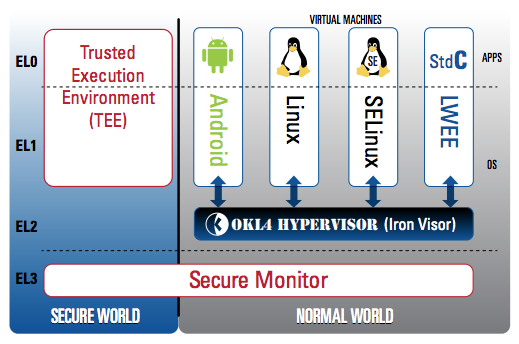
\includegraphics[width=0.65\textwidth]{recursos/OK_L4_Microvisor.png}
	\caption{Arquitectura basada en OKL4 Hypervisor}
	\label{fig:OK_L4_Microvisor}
\end{figure*}
OKL4 Hypervisor proporciona además de servicio a sistemas operativos guest como Linux, VxWorks y Android, un entorno denominado \textit{Lightweight Execution Environments}, que viene a ser un entorno que ofrece rendimentos cercanos a sistemas baremetal.\\
Este hipervisor tiene como uno de sus objetivos principales la seguridad \cite{okl4_2} y se hace mucho énfasis en la confiabilidad que proporciona su sistema frente a ataques externos debido al aislamiento proporcionado entre celdas. También destaca su manejo de los recursos a fin de consumir la mínima de energía, haciéndolo apto para sistemas que funcionan con batería. En la figura \ref{fig:OK_L4_Microvisor} se muestra un ejemplo de arquitectura de sistema basada en OKL4.


\section{WindRiver Hypervisor}
El hipervisor de WindRiver \cite{windriver_1} es también de tipo 1 y particiona el software que se ejecuta en uno o varios núcleos, en múltiples tarjetas virtuales (Virtual Boards) con diferentes niveles de protección y características. Está optimizado para ejecutar sistemas operativos guest de propósito general (\acrshort{GPOS}), sistemas de tiempo real (\acrshort{RTOS}) y sistemas operativos para aplicaciones críticas de seguridad.
\subsection{Virtual Boards}
La división del sistema propuesta por WindRiver se basa en tarjetas virtuales o particiones. Cada una de ellas puede contener un sistema operativo guest con sus diferentes aplicaciones ejecutándose o un programa sin sistema operativo, lo que se denomina \textit{virtual board application}. El hipervisor es el encargado de controlar en qué núcleos se están ejecutando las virtual boards y las zonas de memoria a las que puede acceder. Una virtual board puede compartir un núcleo con otra virtual board, tener un núcleo dedicado, o utilizar varios al mismo tiempo.
\begin{figure*}[h]
	\centering
	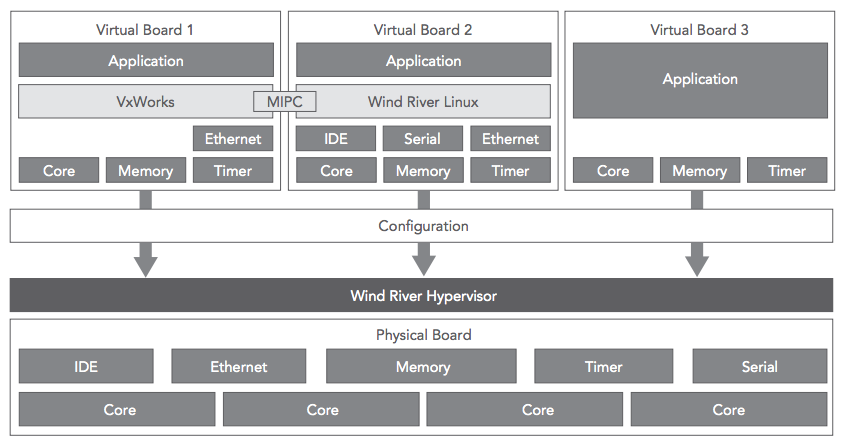
\includegraphics[width=0.75\textwidth]{recursos/windriver_hyp.png}
	\caption{WindRiver Hypervisor}
	\label{fig:windriver_hyp}
\end{figure*}

Las virtual boards pueden ser creadas, arrancadas, detenidas y relanzadas individualmente. Esto porporciona la opción de escalar dinámicamente la aplicación en función de la demanda en cada momento.

\subsection{Sistemas operativos guest}
El hipervisor de WindRiver es capaz de ejecutar sistemas operativos utilizando una mezcla de virtualización asistida por hardware y paravirtualización con el objetivo de proporcionar un rendimiento óptimo. Admite sistemas operativos guest como VxWorks o WindRiver Linux, y proporciona una interfaz para que otros sistemas operativos puedan ejecutarse, incluyendo sistemas operativos de código abierto o licenciados.\\

\paragraph{Sistemas operativos sin modificaciones} El hipervisor de WindRiver permite la ejecución de sistemas operativos sin modificaciones de código del tipo Red Hat Enterprise Linux o Microsoft Windows dentro de una virtual board en microprocesadores Intel con extensiones de virtualización.\\

\paragraph{Sistemas baremetal}
El hipervisor permite la ejecución de virtual boards que no tengan sistema operativo denominadas \textit{bare metal executives}. Hay ciertas tareas en los sistemas embebidos que no requieren de las capacidades que ofrece un sistema operativo, ni de la complejidad que añade. WindRiver proporciona una API abierta, con la que presenta a estas virtual boards la forma de acceder a los recursos del sistema, como la \acrshort{MMU}, excepciones e interrupciones, núcleos de CPU y otros dispositivos necesarios para operar. Esta API permite beneficiarse de las capacidades de la virtualización mientras se mantiene la respuesta en tiempo real necesaria por la aplicación.

\paragraph{Paravirtualización y virtualización asistida por hardware}
Como se ha mencionado anteriormente, muchas familias actuales de microprocesadores proporcionan mecanismos hardware para asistir a la virtualización. El hipervisor de WindRiver se vale de estos mecanismos para proporcionar servicios de virtualización. De la misma manera, existen muchos dispositivos que no proporcionan esta asistencia por hardware, y esos servicios de virtualización los proporciona el software, impactando en el rendimiento del sistema. Para esos casos, se requiere de paravirtualización del sistema operativo.\\
La paravirtualización es la modificación de las llamadas privilegiadas de un sistema operativo para que colabore con el hipervisor. Es este el que debe ejecutar las llamadas privilegiadas en representación del sistema operativo guest. La cantidad de modificaciones necesaria depende mucho de la arquitectura del microprocesador y típicamente implica lo siguiente:

\begin{itemize}
  \item Niveles privilegiados: un sistema virtualizado requiere normalmente de tres niveles de privilegio distintos: uno para el hipervisor, otro para el sistema operativo guest y otro para las aplicaciones. Las arquitecturas de microprocesadores que no proporcionan aistencia por hardware suelen tener solo dos niveles de privilegio. La tarea de la paravirtualización es emular el nivel que falta. Las instrucciones privilegiadas tienen que ser sustituidas por llamadas a la API del hipervisor.
  \item Acceso a dispositivos: un driver en un sistema operativo que se ejecuta nativamente puede acceder a cualquier dispositivo. En un entorno virtualizado, el hipervisor es el que arbitra y decide si una determinada virtual board tiene acceso a un dispositivo o no. Esto incluye interrupciones, dispositivos de entrada salida, registros, y acceso directo a memoria (DMA)
  \item \acrshort{MMU}: el hipervisor controla la \acrshort{MMU} en un entorno virtualizado. Algunos procesadores con asistencia hardware permiten a un sistema guest modificar la \acrshort{MMU} de la virtual board. Si no se dispone de la asistencia hardware, el guest debe colaborar con el hipervisor para modificar la \acrshort{MMU}.
\end{itemize}

\paragraph{Acceso a dispositivos}
El hipervisor de WindRiver proporciona un modelado de dispositivo que permite asignar dispositivos a las virtual boards de diferentes maneras. El acceso al dispositivo puede ser directo, compartido, virtualizado o emulado. Cada una de estas formas de acceder tiene sus particularidades y la elección depende en gran medida de la aplicación y del rendimiento necesario.

\begin{itemize}
  \item Directo: en este modo, el dispositivo es mapeado directamente al espacio de memoria del sistema guest, teniendo este el control exclusivo sobre el dispositivo y no utilizando ninguna característica de la virtualización. El resto de sistemas guest no detectan la existencia del dispositivo. Este modo proporciona el mayor rendimiento posible de acceso.

  \item Compartido: El acceso compartido es deseable cuando un sistema guest de alguna forma posee el acceso al dispositivo (configuración por ejemplo) pero otro sistema guest está interesado en los datos que se producen en dicho dispositivo como se muestra en la figura \ref{fig:windriver_drv_1}.
  \begin{figure*}[!htb]
  	\centering
  	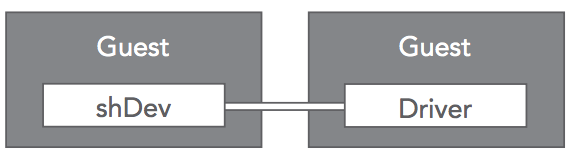
\includegraphics[width=0.65\textwidth]{recursos/windriver_drv_1.png}
  	\caption{Acceso compartido a dispositivo en WindRiver Hypervisor}
  	\label{fig:windriver_drv_1}
  \end{figure*}

  \item Virtualizado: este tipo de acceso se utiliza cuando más de un sistema guest requiere de acceso a un dispositivo (figura \ref{fig:windriver_drv_2}). De esta forma, el driver propiamente dicho se encuentra dentro del hipervisor y los sistemas guest utilizan un driver ``stub'' para comunicarse con él.
  \begin{figure*}[!htb]
  	\centering
  	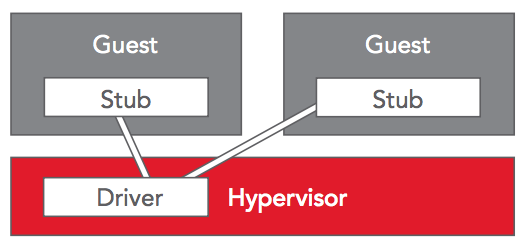
\includegraphics[width=0.65\textwidth]{recursos/windriver_drv_2.png}
  	\caption{Acceso virtualizado a dispositivo en WindRiver Hypervisor}
  	\label{fig:windriver_drv_2}
  \end{figure*}

  \item Emulado: el caso de uso para este tipo de acceso a dispositivo es en el que los drivers de los sistemas guest no pueden ser sustituidos por un driver ``stub''. El hipervisor proporciona una emulación hardware al driver nativo del sistema guest pero por debajo utiliza su propio driver para accedes físicamente al dispositivo (figura \ref{fig:windriver_drv_3}). Los dispositivos emulados ofrecen la mayor de las flexibilidades para las virtual boards pero el impacto en el rendimiento es significativamente mayor que en el resto de los casos.
  \begin{figure*}[!htb]
  	\centering
  	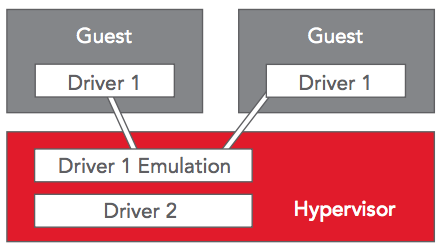
\includegraphics[width=0.65\textwidth]{recursos/windriver_drv_3.png}
  	\caption{Acceso emulado a dispositivo en WindRiver Hypervisor}
  	\label{fig:windriver_drv_3}
  \end{figure*}

\end{itemize}

\paragraph{Comunicaciones entre guests}
El hipervisor de WindRiver facilita la comunicación rápida entre virtual boards proporcionando mensajería punto a punto, comunicación entre procesos multi sistema operativo (\acrshort{MIPC}), y comunicaciones IP, usando un controlador virtual de red (VNIC). Existen dos formas de transporte de mensajes: memoria compartida para conexiones \acrshort{MIPC} y sistema seguro de transporte tanto para conexiones \acrshort{MIPC} como para conexiones \acrshort{VNIC}. Las conexiones rápidas por IP entre virtual boards se consiguen utilizando el driver \acrshort{VNIC} del sistema guest y creando uno o más switches ethernet virtuales dentro del hipervisor.
\begin{figure*}[!htb]
  \centering
  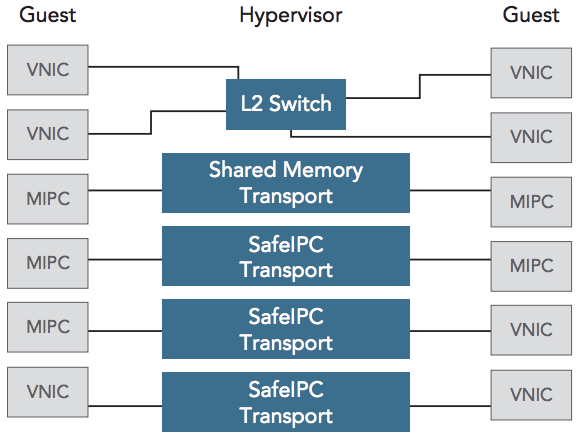
\includegraphics[width=0.65\textwidth]{recursos/windriver_com.png}
  \caption{opciones de comunicación entre virtual boards en WindRiver Hypervisor}
  \label{fig:windriver_com}
\end{figure*}

\section{KVM}
KVM, o \textit{Kernel-based Virtual Machine} \cite{kvm_list}, es un hipervisor de tipo 2, lo que implica que necesita un sistema operativo host para funcionar. Aunque su uso en sistemas embebidos no parece a priori muy adecuado,
se ha introducido en este apartado del documento debido a que es el hipervisor que está en la línea principal de Linux, por lo que tiene detrás una potente fuerza de desarrollo y de usuarios.\\
KVM permite la ejecución de distintos sistemas operativos sin requerir modificaciones en los mismos y tiene versiones para las arquitecturas x86, x86\_64, MIPS, PowerPC y ARM con distintos grados de oficialidad.


\paragraph{Orígenes}
KVM fue anunciado por su creador, Avi Kivity, en octubre de 2006 \cite{kvm_2}. El desarrollo de KVM empezó dentro de la compañía donde trabajaba Kivity, la israelí Qumranet, con el objetivo de corregir las limitaciones de la versión de Xen existente con la que estaban trabajando. En aquel momento, las extensiones de virtualización estaban anunciadas, pero no existían en las arquitecturas de microprocesadores. El desarrollo de KVM se basó en sacar partido a esa tecnología que estaba por llegar y que Xen todavía no incluía. En la arquitectura x86, tradicionalmente el nivel más alto de privilegio era el \textit{ring 0} y para poder ejecutar varios sistemas operativos concurrentemente hacía falta un nivel de privilegio superior a este. Con la irrupción de la tecnología de virtualización de Intel VT-x apareció un conjunto de instrucciones VMX (Virtual Machine Extensions) que introdujo un nivel de privilegio nuevo, \textit{ring -1}, en el que el hipervisor se ejecuta. La primera versión de KVM incluía la utilización de las instrucciones VMX de Intel y pronto incorporó las instrucciones SVM de AMD. En Diciembre de 2006, KVM se integró en la línea principal del kernel de Linux, y la primera versión en la que apareció fue en la 2.6.20 de Febrero de 2007.

\paragraph{Implementación en ARM}
Adelantando la arquitectura de microprocesador que se va a utilizar para el desarrollo del presente trabajo, se va a tener en cuenta únicamente la implementación de KVM en la arquitectura ARM, ya que tiene varias particularidades.\\
El trabajo de adaptar KVM para plataformas basadas en ARM no es sencillo ya que fue concebido para Intel VT-x y difiere en aspectos importantes de la asistencia a la virtualización que ofrece la arquitectura ARM, más concretamente en ARMv8 \cite{kvm_1}.\\
Más adelante se detallarán las características de la asistencia a la virtualización (extensiones de virtualización según ARM \cite{armv8_el}), pero resumiendo, la clave para dar cabida a la virtualización en la arquitectura ARM es la inclusión de un nuevo nivel de privilegio en la CPU, o nivel de excepción (EL) en la nomenclatura ARM. Este nuevo nivel de excepción, EL2, se añade a los ya existentes de usuario y de kernel, EL0 y EL1 respectivamente.
El software que se ejecuta en EL2 puede configurar el hardware para asistir a las máquina virtuales. El hipervisor es el software que se ejecuta en EL2 y que habilita las funciones de virtualización del hardware para permitir a los sistemas guest interactuar mediante una interfaz igual a lo que sería una máquina real. De esta forma, no hace falta modificar los sistemas guest para poder ejecutarse. Los sistemas guest pueden ser ejecutados como si fueran nativos, utilizando EL1 y EL0 hasta que alguna condición hace que se requiera del hipervisor. En este punto, el hardware pasa a EL2, dando control al hipervisor, que puede interactuar directamente con el harware, y finalmente devolver el control al sistema guest.\\
Los hipervisores de tipo 1 encajan bien con este reparto de los niveles de excepción descritos, mientras que los de tipo 2, como KVM, lo tienen más complicado, como se puede apreciar en la figura \ref{fig:kvm_and_xen}:

\begin{figure*}[!htb]
  \centering
  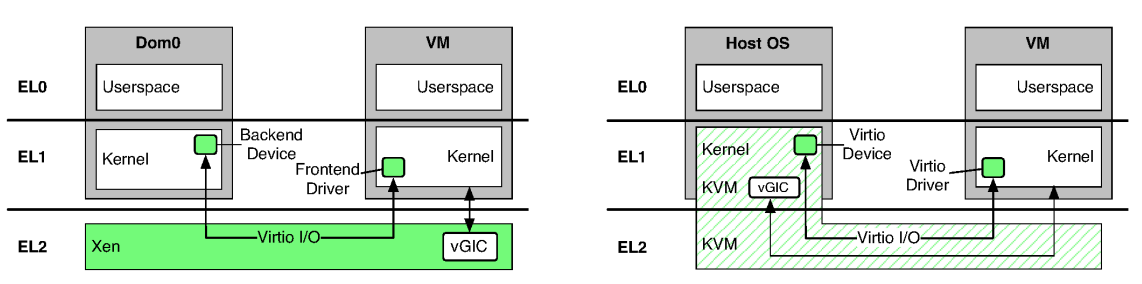
\includegraphics[width=0.95\textwidth]{recursos/kvm_xen_1.png}
  \caption{Xen y KVM en ARMv8}
  \label{fig:kvm_and_xen}
\end{figure*}

Los sistemas operativos existentes están diseñados para ejecutarse en EL1, así que un hipervisor de tipo 2, que necesita de un sistema operativo host (KVM y Linux en este caso) para ejecutarse y acceder al hardware
no encaja tan bien en la arquitectura ARMv8. El EL2 es estrictamente un nivel de excepción mayor que EL1 con registros diferentes. Cambiar Linux para que se ejecute en EL2 requiere de demasiadas modificaciones que no serían prácticas, por tanto, KVM se ejecuta tanto en EL1 como en EL2 en un modo denominado virtualización partida, o \textit{split-mode virtualization}. De este modo, por un lado se comparte el EL1 entre el sistema operativo host (Linux) y las máquinas virtuales, y, por otro, se utiliza EL2 para habilitar las extensiones de virtualización que permitan ejecutar las máquinas virtuales con un rendimiento cercano al de un sistema nativo. KVM habilita estas extensiones en EL2 cuando se cambia de modo host a modo máquina virtual, y las deshabilita cuando vuelve a cambiar a host. De esta forma se podría decir que una máquina virtual ejecutándose con KVM, no es más que otro proceso más para el sistema operativo host, lo que requiere un cambio de contexto cuando se entra y se sale de la máquina virtual.\\


\section{Xen}
Xen \cite{xen_arm_whitepaper} es un hypervisor de tipo 1 de código abierto que se ejecuta directamente sobre el hardware. Todo lo demás son máquinas virtuales que se ejecutan por encima de Xen, incluido el denominado Dom0. En la nomenclatura de Xen, un dominio es equivalente a una máquina virtual. El Dom0 es la primera máquina virtual y se crea durante el arranque por Xen. Se trata de una máquina virtual con privilegios especiales que maneja los dispositivos de la plataforma.\\
Xen virtualiza la CPU, la memoria, las interrupciones y los temporizadores. De esta forma, proporciona a las máquinas virtuales una o más CPUs virtuales, una parte de la memoria del sistema, un controlador virtual de interrupciones y un temporizador virtual. En su configuración por defecto, Xen asigna dispositivos, como controladores SATA o tarjetas de red, al Dom0, teniendo en cuenta la recolocación de zonas MMIO e interrupciones. El Dom0 utiliza el mismo driver de dispositivo que si se estuviera ejecutando de forma nativa, sin hipervisor. Este dominio normalmente es Linux aunque podría ser FreeBSD u otro sistema operativo.\\
El Dom0 también dispone de una serie de drivers, denominados \textit{paravirtualized backends}, para dar acceso al disco, red, etc. al resto de máquinas virtuales no privilegiadas, denominadas DomU por en Xen. Estas pueden obtener acceso a una serie de dispositivos virtuales genéricos a través de los correspondientes drivers \textit{paravirtualized frontends}. Generalmente, existe una pareja de drivers \textit{paravirtualizados} para los dispositivos más comunes, como discos de almacenamiento, controladores de red, puerto serie, framebuffer, ratón, teclado, etc. Normalmente, están alojados en el kernel, aunque algunos pueden ejecutarse desde espacio de usuario en QEMU. Los drivers \textit{frontend} conectan con los drivers \textit{backend} mediante un sencillo protocolo en anillo sobre una página de memoria compartida. Xen proporciona todas las herramientas para el descubrimiento y establecimiento inicial de la comunicación. También proporciona un mecanismo para compartir páginas adicionales y enviar notificaciones usando interrupciones software \cite{xen_arm_whitepaper}.\\

\begin{figure*}[!htb]
  \centering
  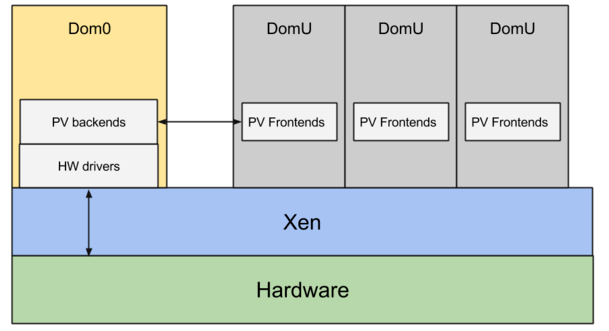
\includegraphics[width=0.70\textwidth]{recursos/xen_1.png}
  \caption{Arquitectura típica de Xen}
  \label{fig:xen_1}
\end{figure*}

Aunque la configuración representada en la figura \ref{fig:xen_1} es la más utilizada, no es obligatorio que todos los drivers de dispositivos y todos los \textit{backends} se ejecuten en el Dom0. La arquitectura Xen permite lo que se denominan dominios de drivers. Estos son máquinas virtuales sin privilegios, cuyo único objetivo es servir de \textit{backend} y ejecutar el driver correspondiente a una única clase de dispositivo, como se puede observar en la figura \ref{fig:xen_2}.\\

\begin{figure*}[!htb]
  \centering
  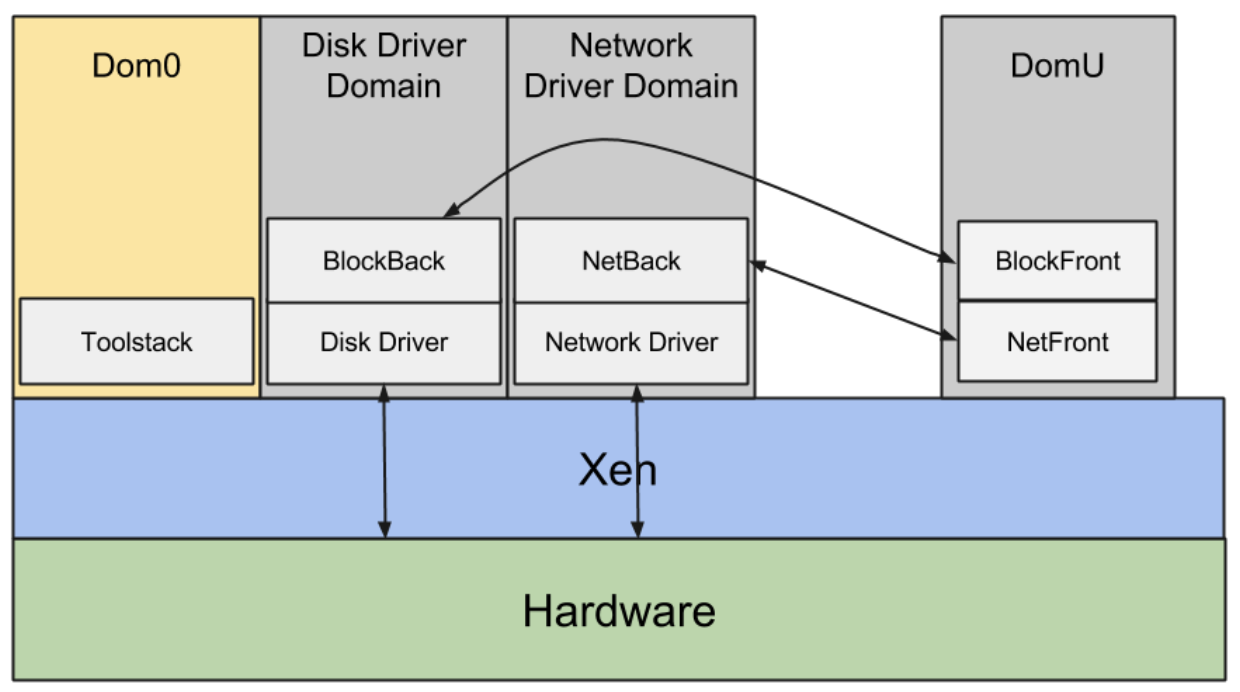
\includegraphics[width=0.70\textwidth]{recursos/xen_2.png}
  \caption{Dominios de drivers en Xen}
  \label{fig:xen_2}
\end{figure*}

Con esta configuración, por ejemplo, se puede disponer de un dominio de driver de red al que se le asigna la tarjeta de red del sistema. En este dominio se ejecuta el driver del dispositivo de red y también el \textit{backend} que se expone al resto de dominios. Ya que los dominios de dispositivos son normales, sin privilegios, es posible ejecutar gran parte de código, como la pila de protocolos de comunicaciones, en máquinas virtuales sin privilegios. Incluso en el caso de que un usuario malintencionado ganara acceso al dominio del driver de red, no podría hacer caer el sistema completo, debido al aislamiento existente entre dominios. Esta forma de configurar Xen permite una gran flexibilidad a la hora de discretizar sistemas complejos en componentes aislados.

\subsection{Xen en ARM}
\subsubsection{Arquitectura}

La implementación de Xen en ARM difiere en gran medida de la que existe para las arquitecturas x86. Originalmente, Xen se desarrolló para arquitecturas Intel x86 y tuvo que ser portado para ARM. Los desarrolladores aprovecharon la ocasión para deshacerse de muchas líneas de código que ya no eran útiles y se habían ido acumulando con los años en el desarrollo. Una de las características que eliminaron fué la emulación, ya que las iterfaces emuladas son lentas e inseguras. QEMU, usado para la emulación en la versión de Xen para x86, a pesar de ser un código que goza de buena salud y mantenido por la comunidad de software de código abierto, es demasiado grande, tanto en líneas de código como en tamaño de ejecutable. A la hora de portar Xen a ARM se optó por hacerlo cuanto más sencillo y más pequeño mejor. Por ese motivo, QEMU no está presente. En su lugar, se trata de aprovechar las extensiones de virtualización del hardware tanto como es posible y utilizar interfaces \textit{paravirtualizadas} para dispositivos de entrada y salida. Como resultado de esto, Xen en ARM es más rápido y seguro \cite{xen_arm_whitepaper}.

\subsubsection{Xen y ARMv8}

Las extensiones de virtualización de ARM resultan muy adecuadas para la arquitectura de Xen:
\begin{itemize}
  \item Xen se ejecuta por completo en el nivel de excepcion de hipervisor.  Xen deja el EL1 para el modo kernel del sistema operativo de la máquina virtual y el EL0 para para las aplicaciones de usuario. Al ejecutarse completamente en EL2, Xen permite reducir el número de cambios de contexto necesarios entre modo hipervisor y modo kernel.
  \item La inclusión de la intrucción HVC, permite al kernel invocar \textit{hypercalls} hacia Xen.
  \item Xen utiliza 2 fases en la \acrshort{MMU} para asignar memoria a las máquinas virtuales.
  \item Se emplean temporizadores genéricos tanto para recibir interrupciones de tiempo como para inyectarlas en las máquinas virtuales.
  \item Xen configura en GIC las interrupciones necesarias tanto para su funcionamiento como para inyectar interrupciones en los sistemas guest.
\end{itemize}

\begin{figure*}[!h]
  \centering
  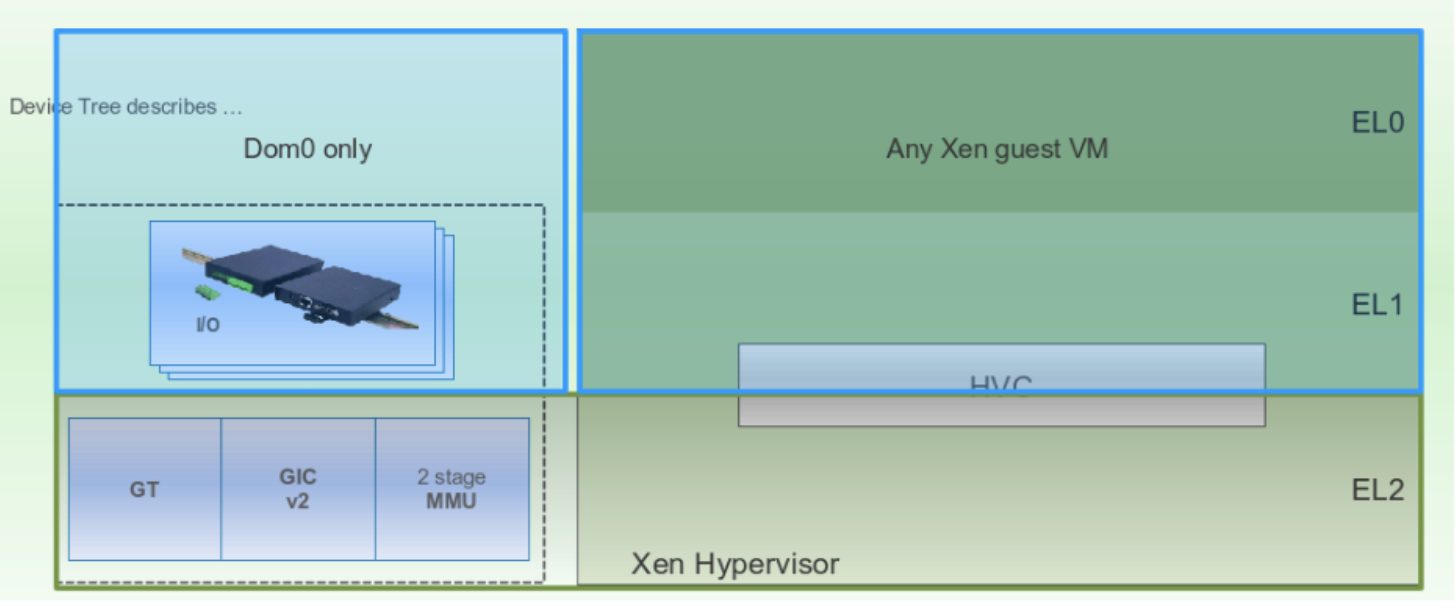
\includegraphics[width=0.90\textwidth]{recursos/xen_3.png}
  \caption{Xen en ARMv8}
  \label{fig:xen_3}
\end{figure*}

El Dom0 arranca exáctamente igual que lo haría nativamente. Usa el \textit{device-tree} para descubrir el hardware (en caso de Linux u otros Dom0 que se basen en \textit{device-tree}) y carga los drivers correspondientes. Al encontrarse con el nodo de hipervisor, el Dom0 es consciente de que se está ejecutando sobre Xen y puede inicializar los \textit{backends} que se necesiten.

\subsubsection{Tamaño del código}

Debido al buen acople entre la arquitectura de Xen y las extensiones de virtualización de ARMv8 y a la limpieza de código de x86 efectuada, el tamaño de Xen para ARM ha resultado ser una sexta parte de lo que existe para x86\_64 como se aprecia en la tabla \ref{table:results45}.

\begin{table}[!ht]
  \centering
	\begin{tabular}{ |c|c|c|c|c| }
		\hline
     & Common & ARMv7 & ARMv8 & Total\\
    \hline
    xen/arch/arm          & 11,767      & 3,503  & 1,812   & 17,082 \\
    \hline
    C                     & 11,587      & 954    & 813	    & 13,354 \\
    \hline
    ASM                   & 180         & 2,549  & 999     & 3,728  \\
    \hline
    xen/include/asm-arm   & 4,786       & 984    & 1,050   & 6,820  \\
    \hline
    Total ARM	            & 16,553  & 4,487  & 2,862        & 23,902 \\
    \hline
    \multicolumn{4}{|c|}{x86\_64}                           & Total\\
    \hline
    \multicolumn{4}{|c|}{xen/arch/x86}                      & 124,615\\
    \hline
    \multicolumn{4}{|c|}{xen/include/asm-x86}               & 18,530 \\
    \hline
    \multicolumn{4}{|c|}{Total x86\_64}                     & 143,145\\
    \hline
	\end{tabular}
	\caption{Número de lineas de código de Xen versión 4.4.0 en ARM y x86 \cite{xen_arm_whitepaper}}
  \label{table:results45}
\end{table}

\section{Jailhouse} \label{jailhouse_sota}

En primer lugar, Jailhouse \cite{jailhouse_elc2017} se declara más preocupado del aislamiento y segmentación que de la virtualización \cite{jailhouse_p1}. Se denomina \textit{hipervisor de particionamiento estático} y es de tipo 1. Está diseñado para cooperar con Linux y ejecutar aplicaciones baremetal u otros sistemas operativos guest. Jailhouse es muy ligero y no proporciona muchas de las funciones que tradicionalmente proporcionan los hipervisores, como puede ser la sobreutilización de recursos. Por ejemplo no ofrece vCPUs a los sistemas guest y no emula dispositivos que no tiene, por lo que no necesita de un scheduler que vaya repartiendo los recursos en cada momento. La idea principal detrás de Jailhouse es mantener el hipervisor lo más sencillo posible. Su desarrollo empezó en 2013 así que se trata de un hipervisor relativamente nuevo. El soporte para la arquitectura ARMv8 no fue incorporado a la rama principal de desarrollo hasta enero de 2017.\\

\begin{figure*}[h]
  \centering
  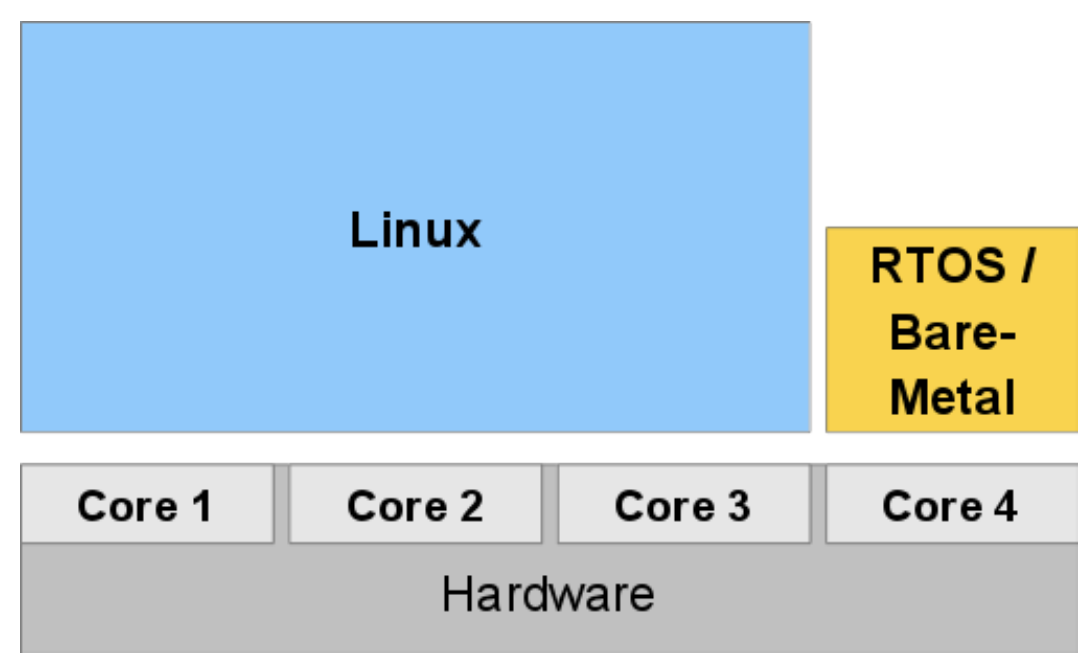
\includegraphics[width=0.80\textwidth]{recursos/jailhouse_1.png}
  \caption{Configuración típica de Jailhouse}
  \label{fig:jail_1}
\end{figure*}

Jailhouse habilita el multiprocesamiento asímetrico (\acrshort{AMP}) desde Linux y divide el sistema en particiones aisaldas llamadas ``celdas''. Cada celda ejecuta un sistema guest y tiene una serie de recursos asignados (núcleos, zonas de memoria, dispositivos) que controla totalmente. El trabajo del hipervisor es gestionar las celdas y mantener el aislamientro entre ellas. Jailhouse basa su funcionanmiento principalmente en las extensiones de virtualización de las arquitecturas x86 y ARM, que son las que admite actualmente.\\
Un sistema que utiliza Jailhouse debe tener al menos una celda Linux que es la que arranca primero. En esta celda existe un módulo del kernel que lanza el hipervisor y tambien están las herramientas para crear, lanzar, parar y destruir las diferentes celdas. El rol de esta celda es parecido al Dom0 de Xen. Una vez creada una celda, la celda Linux pierde el conocimiento del núcleo o núcleos en el que se crea. De manera similar, los programas ejecutándose en una celda no son conscientes de que están en una máquina virtual, ni conocen la existencia de núcleos fuera de esa celda. El proceso de arranque se puede apreciar en la figura \ref{fig:jail_2}:\\

\begin{figure*}[h]
  \centering
  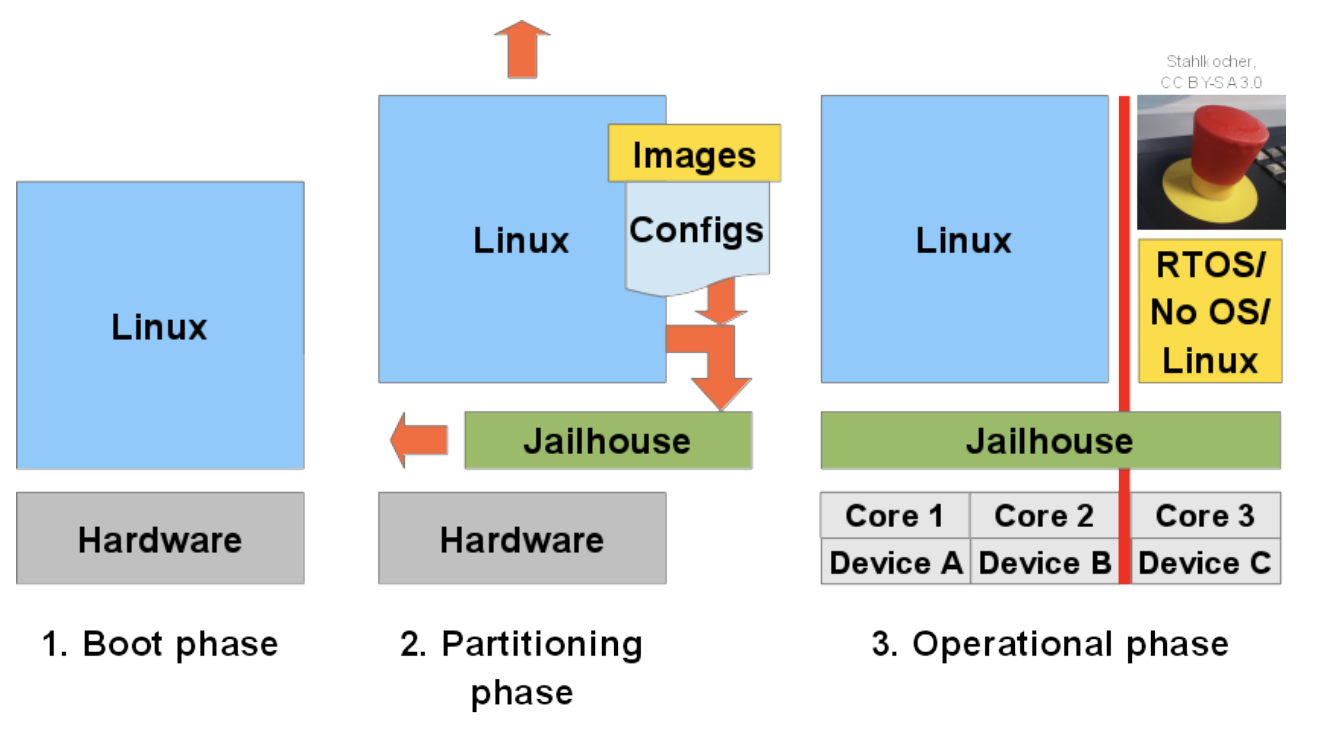
\includegraphics[width=0.80\textwidth]{recursos/jailhouse_2.png}
  \caption{Particionamiento del sistema en Jailhouse}
  \label{fig:jail_2}
\end{figure*}
